%region Verzování
\chapter{Verzování}
\label{sec:versioning}
Tato kapitola se věnuje verzování softwaru a jeho významu pro vývoj a~údržbu projektů. Dále je popsán konkrétní verzovací nástroj Git, jeho funkce a~programovatelný přístup k~jeho datům.

%region Verzování softwaru
\section{Verzování softwaru}
\label{sec:versioning_software}
Verzování je proces správy a~sledování změn v~projektu~\cite{ernst2024vcs}. V~tomto procesu se uchovává kompletní historie veškerých změn souborů, které jsou verzovány. Nejčastěji se takovéto nástroje používají u~textových zdrojových kódů softwaru, avšak lze je využít pro libovolné typy souborů.

\VCS obvykle eviduje, kdo změnil jaký soubor a~co konkrétního v~tom souboru změnil. Díky tomu lze kdykoliv dohledat, kdo napsal jakou část kódu, případně proč byla tato část změněna~\cite{sink2011version}. Na základě těchto informací lze u~\VCS snadno vrátit zpět změny, které se ukázaly jako nevhodné.

\VCS řeší také problém správy verzí, kdy před jeho zavedením bylo nutné uchovávat mnoho kopií téhož projektu s~různými popisky identifikujícími jejich verzi, což vyžadovalo nadměrnou disciplínu a~výrazně více úložného prostoru. U~\VCS jsou zpravidla ukládány pouze skutečné změny oproti předchozí verzi, nikoli celá kopie projektu, přičemž vše je spravováno interně daným nástrojem a~uživateli tak odpadá starost s~organizací a~ukládáním jednotlivých verzí.

Další vlastností \VCS je možnost souběžné práce více uživatelů na stejných souborech. \VCS umožňuje řešit konflikty (tzv.\ \textit{merge konflikty}), které vznikají při souběžné úpravě stejného souboru více uživateli~\cite{sink2011version}.

\customref{Na obrázku}{fig:revision_controlled_project_visualization} je znázorněn příklad typické struktury historie projektu řízeného verzovacím systémem. Základní ideální struktura je lineární graf, tj.\ řada uzlů za sebou, kde každý další vychází z~předchozího. Projekt má hlavní větev (Trunk), z~níž se dále větví ostatní větve (Branches), například pro vývoj nové funkcionality. Větve se poté slučují zpět (Merges) a~vznikají nové verze projektu. Z~pohledu teorie grafů se jedná o~acyklický orientovaný graf. Může se stát, že nově vyvíjená funkcionalita je nevyhovující, a~tak vzniká slepá větev (Discontinued development branch). Jakmile je dosažen požadovaný stav v~hlavní větvi, provádí se tzv.\ tagování (Tags). Tag většinou označuje novou verzi projektu nebo jiný důležitý milník.

\begin{figure}[ht]
  \centering
  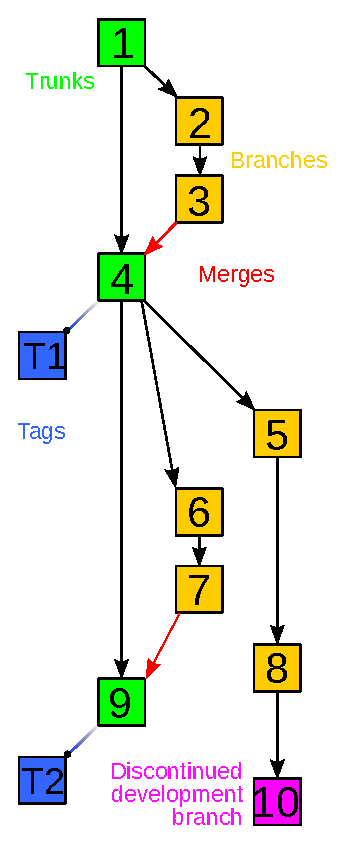
\includegraphics[height=\textwidth]{figures/vcs/Revision_controlled_project_visualization.pdf}
  \caption{Příklad historie projektu řízené verzovacím systémem~\cite{sink2011version}.}
  \label{fig:revision_controlled_project_visualization}
\end{figure}

%endregion

%region Centrální vs. distribuované VCS
\subsection{Centrální vs.\ distribuované VCS}
\label{sec:vcs_types}
Hlavní rozdíl mezi centrálními a~distribuovanými \VCS spočívá v~tom, že distribuované \VCS uchovávají kopii kompletní historie změn jak u~každého uživatele, tak i~na hostovacím serveru~\cite{sink2011version}.

\customref{Na obrázku}{fig:vcs_comparison} jsou zobrazeny oba typy architektury. U~centrálního \VCS se musí spoléhat výhradně na hostovací server. Pokud ten vypadne, v~lepším případě uživatelé nemohou publikovat své změny, v~horším případě při absenci zálohy dojde ke ztrátě celé historie. U~distribuovaného \VCS stačí, aby alespoň jeden uživatel měl projekt k~dispozici, protože každý uživatel s~lokální kopií projektu disponuje prakticky plnohodnotnou zálohou s~kompletní historií a jednoduše se může projekt obnovit nebo znovu nasadit na jakoukoli jinou hostovací službu.

\begin{figure}[ht]
  \centering
  \subfloat[Centralizované VCS]{\label{fig:centralized_vcs}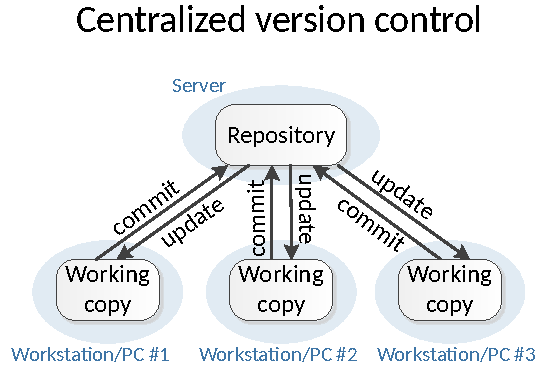
\includegraphics[width=0.45\textwidth]{figures/vcs/central-version-control.pdf}}
  \hfill
  \subfloat[Distribuované VCS]{\label{fig:distributed_vcs}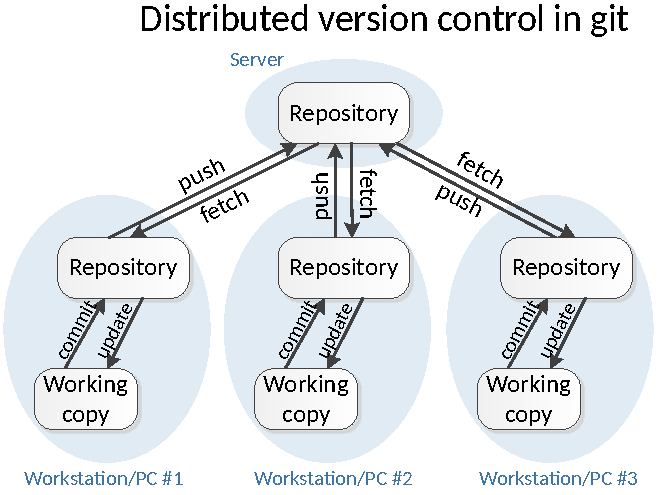
\includegraphics[width=0.45\textwidth]{figures/vcs/distributed-version-control.pdf}}
  \caption{Porovnání centralizované a distribuované architektury verzovacích systémů~\cite{sink2011version}.}
  \label{fig:vcs_comparison}
\end{figure}

Rozdíl je patrný i~v~principu odesílání změn. U~centrálního \VCS příkaz \code{svn commit} zapíše změny přímo na server, zatímco u~distribuovaného \VCS (v~případě Gitu) příkaz \code{git commit} provede změny pouze do lokálního repozitáře. Teprve příkaz \code{git push} odešle všechny dosud lokálně zapsané, avšak nepropagované commity na hostovací službu. Tedy u~centrálního \VCS je vyžadováno připojení k~serveru pro publikování změn, zatímco u~distribuovaného není vyžadováno a můžeme změny na server zapsat později.

Za zmínku dále stojí, že příkaz \code{git pull} ve skutečnosti zastřešuje dvě operace: nejprve stáhne změny ze serveru a~poté je sloučí s~lokálními změnami. Není tedy přímým opakem příkazu \code{git push}.

Rozdíl je patrný i~v~principu řešení konfliktů a~slučování větví. Centralizovaný \VCS umožňuje provést aktualizaci ze serveru, i~když má uživatel rozpracované, dosud nezapsané soubory, a~systém automaticky smíchá všechny změny, což může vést ke konfliktům. Distribuovaný \VCS uživatele nejprve donutí provést \code{commit}, čímž se změny zapíší do lokální historie, a~teprve poté se může provést \code{merge} mezi dvěma pevnými body historie, z~nichž vzniká nový pevný bod historie.

%endregion

%endregion
